%!TEX root = ../thesis.tex

\chapter{Practical performences}
\label{chap:pracPerf}
\section{Setup}
\label{sec:Setup}
In the following chapter we will examine the practical relative performances of the three algorithms. We will do so in several ways. The first way is with the use of simulated data (recreated from \cite{Hastie2009}). We have ten features $X_1,\ldots,X_{10}$ which are drawn from a standard independent Gaussian. Their label is determined (deterministically) by the following rule: $$Y:=\begin{cases}
1 & \text{ if } \sum_{k=0}^{10} (X_k)^2 > \chi_{10}^2(0.5)\\
-1 & \text{otherwise}
\end{cases}$$ Where $\chi_{10}^2(0.5)=9.34$ is the median of a chi-squared random variable with ten degrees of freedom. This is to ensure that there roughly the same amount of labels in each category. 

\par The second way we will test the algorithms is the UCI ``a9a Adult dataset'' \footnote{https://www.csie.ntu.edu.tw/~cjlin/libsvmtools/datasets/binary.html}. Here the goal is to predict whether an individual will earn more than \$50,000 per year or not. The original data set has 14 features, among which six are continuous and eight are categorical. In this data set, continuous features are discretized into quantiles, and each quantile is represented by a binary feature. Furthermore a categorical feature with $m$ categories is converted to $m$ binary features. 

\par The final way we will attempt to compare the algorithms is to give them a fixed amount of CPU time and then compare the number of iterations they were able to do until the time elapsed and their accuracy at that point. Because of practical considerations we allow the algorithms to complete the current iteration when the time runs out, but since a single iteration doesn't take very long this should be of little concern.

\par In an attempt to keep the comparison as consistent as possible we will, in all settings, use 32,561 observations for training and 16,281 for testing. This is because these are the amount of observations in the a9a data set. This ratio of training to testing observations is not uncommon. Recall to avoid over fitting we cannot test the algorithm on the same dataset we use to train it, thus any observations which are used to test cannot be used to train, therefore this kind of ratio is desirable.

\newpage
\section{Datasets}
\subsection{\adaB}
\label{subsec:AdaPracPerf}

\begin{figure}[!ht]
  \centering
      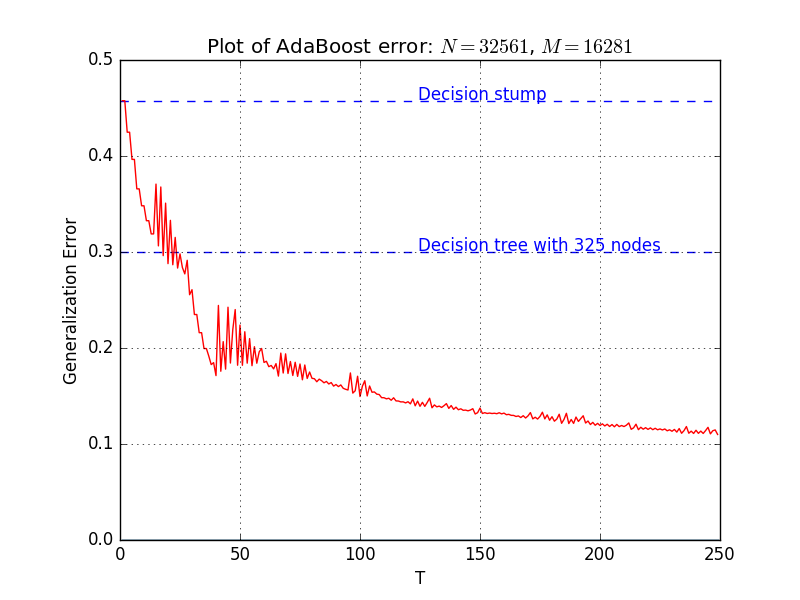
\includegraphics[width=0.8\textwidth]{generated/ADGD.png}
  \caption{Generalization error of AdaBoost as a function of the number of iterations with 10000 examples and test cases. The error of actual stumps and a tree with 217 nodes is also shown for reference.}
      \label{fig:adaB}
\end{figure}

\begin{figure}[!ht]
  \centering
      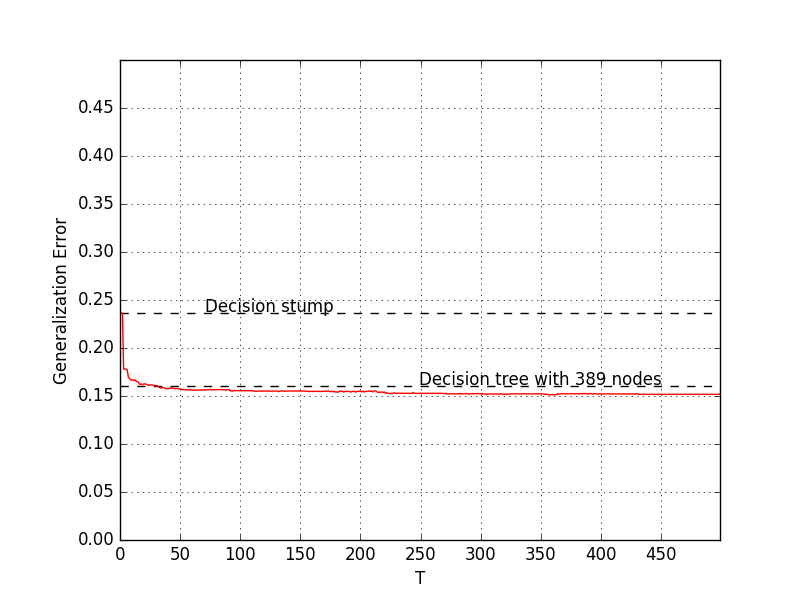
\includegraphics[width=0.8\textwidth]{generated/ADSVM.png}
  \caption{Generalization error of AdaBoost as a function of the number of iterations with 10000 examples and test cases. The error of actual stumps and a tree with 217 nodes is also shown for reference.}
      \label{fig:adaB}
\end{figure}

\begin{figure}[!ht]
  \centering
      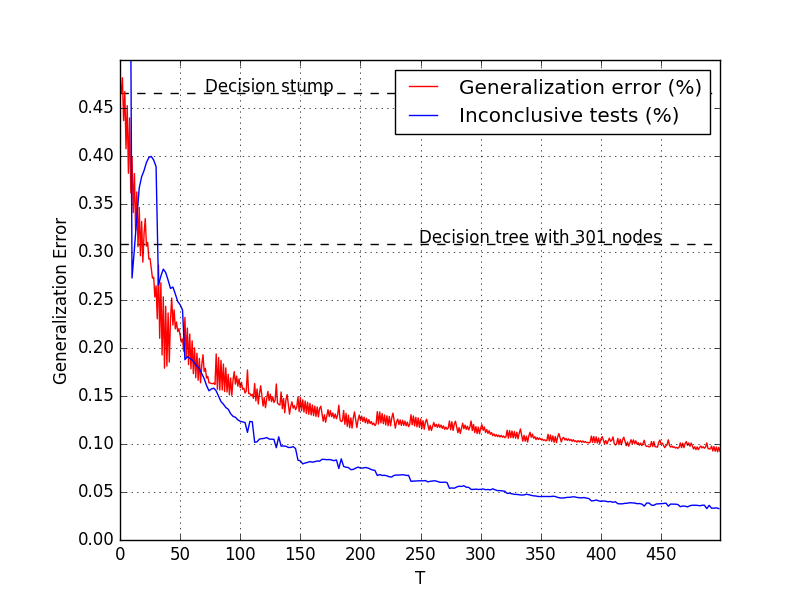
\includegraphics[width=0.8\textwidth]{generated/SQGD.png}
  \caption{Generalization error of AdaBoost as a function of the number of iterations with 10000 examples and test cases. The error of actual stumps and a tree with 217 nodes is also shown for reference.}
      \label{fig:adaB}
\end{figure}

\par Looking at figure \ref{fig:adaB} it is obvious that our algorithm works. The decision stump initially performs with an error rate of 47\% which is indeed only slightly better than random guessing. \adaB outperforms this and even a large tree with 217 nodes and an error rate of 30\% after just tens of iterations and reaches an error rate as low as 8\% after 400 iterations. 

 \subsection{\NHB}
 \label{subsec:NHPracPerf}
\newpage
\section{Computation}
\begin{table}[htbp]
\centering
\begin{tabular}{|c|c|c|c|c|}
\hline
Algorithm & Execution time (s) & Iterations & Error (\%) & Inconclusive tests (\%)  \\ \hhline{|=|=|=|=|=|}
\multirow{ 2}{*}{\adaB} & 1.194 & 5 & 39.64 & 0.00  \\\cline{2-5}
& 60.122 & 241 &  11.11 & 0.00  \\ \Xhline{1pt}
\multirow{ 2}{*}{\adaN} & 1.004 & 220 & 11.48  & 0.0 \\\cline{2-5}
& 60.000 & 15407 &  6.99 & 0.18  \\ \Xhline{1pt}
\multirow{ 2}{*}{\squintB} & 1.002 & 31 & 26.80  & 39.09\\\cline{2-5}
 & 60.022 & 1711 &  7.56  &  1.02\\ \hline
\end{tabular}
\caption{Timed tests of the algorithms on the simulated data}
\label{tbl:GDTime}
\end{table}

\begin{table}[htbp]
\centering
\begin{tabular}{|c|c|c|c|c|}
\hline
Algorithm & Execution time (s) & Iterations & Error (\%) & Inconclusive tests (\%)  \\ \hhline{|=|=|=|=|=|}
\multirow{ 2}{*}{\adaB} & 1.167 & 6 & 17.68 & 0.00  \\\cline{2-5}
& 60.192 & 297 &  15.25 & 0.00  \\ \Xhline{1pt}
\multirow{ 2}{*}{\NHB} & 1.085 & 12 & 17.80  & 0.0 \\\cline{2-5}
& 60.0120 & 578 &  15.14 & 0.0  \\ \Xhline{1pt}
\multirow{ 2}{*}{\squintB} & 1.024 & 15 & 17.93  & 9.23\\\cline{2-5}
 & 60.009 & 815 &  15.23  &  13.81\\ \hline
\end{tabular}
\caption{Timed tests of the algorithms on the a9a data}
\label{table2}
\end{table}

 \section{Conclusion and Future Work}